\documentclass[a4paper]{scrartcl}
\usepackage[utf8]{inputenc}
\usepackage[english]{babel}
\usepackage{graphicx}
\usepackage{amssymb,amsmath}
\usepackage[numbers]{natbib}
\usepackage{listings} \lstset{numbers=left, numberstyle=\tiny, numbersep=3pt}
\usepackage{colortbl}
\usepackage{setspace}
%\usepackage{tabularx}

% old colour scheme - to be replaced
% red
%\definecolor{javared}{RGB}{204,51,63}
% orange
%\definecolor{javagreen}{RGB}{235,104,65}
% darkblue
%\definecolor{javapurple}{RGB}{0,72,79}

%\definecolor{commentgrey}{rgb}{0.2,0.2,0.2}

% new colour scheme
\definecolor{darkblue}{RGB}{0,72,79}
\definecolor{blue}{RGB}{0,160,176}
\definecolor{red}{RGB}{204,51,63}
\definecolor{orange}{RGB}{235,104,65}
\definecolor{yellow}{RGB}{237,201,81}
\definecolor{lightgreen}{RGB}{136,166,94}
\definecolor{green}{RGB}{94,140,106}
\definecolor{brown}{RGB}{106,74,60}
\definecolor{lightgrey}{RGB}{176,176,176}
\definecolor{grey}{RGB}{79,79,79}

% need to define for each listing:
% comment=[l]{//},% define comment
%keywordstyle=\color{red},
%morekeywords={*,...,strvcat}
\lstset{
  captionpos=b,%
  tabsize=2,%
  %comment=[l]{//},% define comment
  commentstyle=\itshape\color{grey},
  morecomment=[l]{//},
  morecomment=[s]{/*}{*/},
  morecomment=[l]{\%},
  mathescape=true,%
  xrightmargin=3.5mm,
  frame=lines,
  framexrightmargin=3.8mm,
  basicstyle=\normalsize\ttfamily,% normal font
  numbers=right,%
  numberstyle=\tiny\ttfamily,% line number font
  breaklines=true,% <-
  breakindent=10pt,%
  numberstyle=\tiny,%
  stepnumber=1,%
  numbersep=5pt,
  showstringspaces=false,        % underline spaces within strings
}


\renewcommand{\familydefault}{\sfdefault}
% allow page breaks in AMS maths eqnarray
\allowdisplaybreaks[1]
\title{TinyRNG - a simplistic random number generation and transformation library\\
{\normalsize Documentation}
}
\author{Guido Klingbeil}
\date{\today}
%
\begin{document}
\setlength{\parindent}{0pt}
\maketitle
\vspace{-2.2cm}
\section*{}

% Introduction
TinyRNG is a very small and simplistic random number generation and transformation library implemented in C. It is built around the two very simple random number generators (RNGs) XORSHIFT and KISS (Keep It Simple Stupid) designed by George Marsaglia. Both pass the BigCrunch battery test of the TestU01 testsuite by \citet{L'Ecuyer2007}.

TinyRNG generates random numbers with 32-bit or 64-bit of randomness and provides transformation into samples from the following distributions:

\begin{itemize}
  \item uniform $[0,1)$,
  \item exponential,
  \item standard normal,
  \item normal,
  \item binomial,
  \item Poisson,
  \item Gamma,
  \item Beta.
\end{itemize}

% general remarks on the interface

TinyRNG uses a strict {\it call by reference} design. Each function returns the integer $0$ on success and a non-zero error code defined in {\sf TinyRNG.h} if it fails. The generated sample is written to an address provided by the user as a C pointer.

The library consists of two distinct parts: (i) the pseudo RNG generating 32-bit or 64-bit random integers, (ii) the transformation algorithms. To make the addition of new RNGs simple, the RNGs are passed as function pointers to the transformation algorithms. The example below demonstrates this. A random integer generated by the 32-bit XORSHIFT RNG {\sf xorshift32} is transformed into a uniformly distributed random sample on the interval $[0, 1)]$ by calling {\sf unifrnd32} with the generator {\sf xorshift32} as a parameter:
 
\begin{lstlisting}[float, caption={Example code generating a uniform random sample on the interval $[0,1)$.}],
  float sample = 0.0f;
  uint32_t err = 0;
  uint32_t *seeds;

  // allocate the seed memory
  seeds = (uint32_t*)malloc(5 * sizeof(uint32_t));

  // seed the RNG
  err = seed(seeds, 5);
 
  // generate a 32-bit uniform [0,1) random sample using the XORSHIFT RNG
  err = unifrnd32(xorshift32, seeds, &fsample);

  // free the allocated memory
  free(seeds);
\end{lstlisting}

A design goal of TinyRNG was to make it thread safe. The state vector seeds of the RNGs are passed as a pointer to the RNGs. Furthermore, non of the transformation algorithms maintains an internal state between function calls.   

% how to extend the library


% reference to the KISS generator:
% http://www.cse.yorku.ca/~oz/marsaglia-rng.html

\label{app:random_number_generation}
While many simulation tasks require a reliable random number generator (RNG), implementing  such a generator is not the main focus of many researchers. However, a simple and at the code level understandable RNG seems to be desirable. The RNG design is chosen to minimise the error possibilities: (i) the implementation is as minimal as possible, (ii) the dependencies between transformations are kept minimal, all of them are transformations of uniform random numbers or normal random numbers. The uniform RNG is tested rigorously with the {\it TestU01} test suite by\,\cite{L'Ecuyer2007}. Our implementations of the transformations are tested by generating 10000 using our implementation and the same number of samples from the same distribution using MATLAB's RNG and testing both sets of random samples using the Kolmogorov-Smirnov-test\,\citep{Dudewicz1988}.

% which uniform random number generator do I use

% extract from ``good practices"
% seeding by reading from /dev/urandom
% do not use the bad library generators
% do not use too many random numbers
% the RNG is easily replacable

\section*{Uniform random number generator}
The uniform RNG generates a sequence of samples uniformly distributed $U(0,1)$ on the interval $(0,1]$ which can easily be re-scaled to the interval $(a, b]$  where $-\infty < a < b < \infty$. The implemented uniform RNG is a member of the XORSHIFT family of generators proposed by\,\citep{Marsaglia2003}. XORSHIFT generators are a special form of the linear feedback shift register (LFSR) generators\,\citep{Brent2004, Panneton2005}. They  are compact, only requiring a very few lines of source-code, and only bit-shift and integer addition operations which are efficiently implemented in hardware.

This section gives a very brief sketch of the XORSHIFT generator's design idea. The starting point is the linear recurrence for fixed values $r > s > 0$:

\begin{equation}
x_{k} = x_{k - r} \mathbf{A} + x_{k - s} \mathbf{B}
\label{app:eqn:xorshift_recurrence}
~,\end{equation}

where $x_k$ is a binary vector, consisting of $\{ 0, 1\}$, of length $w$ and $\mathbf{A}$ and $\mathbf{B}$ are $w \times w$ binary matrices. $w$ is the word length and is typically chosen to match the computer's word length ($w = 32$ or $w = 64$).

Computing vector matrix products is usually regarded as computationally expensive. The core idea of \citet{Marsaglia2003} is to lower the computational burden by assuming that $\mathbf{A} $ and $\mathbf{B}$ are products of small terms $(\mathbf{I} + \mathbf{L}^a)$ and $(\mathbf{I} + \mathbf{R}^b)$ where $\mathbf{L}$ and $\mathbf{R}$ are $w \times w$ shift matrices. The left shift matrix $\mathbf{L}$ is a binary matrix such that $(x_1, \dots, x_w) \mathbf{L} = (x_2, \dots, x_w, 0)$, and the right shift matrix $\mathbf{R}$ is such that $(x_1, \dots, x_w) \mathbf{R} = (0, x_2, \dots, x_{w-1})$. Since, $\mathbf{R} = \mathbf{L}^T$ it is sufficient to give $\mathbf{L}$:

\begin{equation*}
\mathbf{L} = \left( \begin{array}{cccc}
0 & 0 & \dots & 0 \\
1 & 0 & \dots & 0 \\
\vdots & \ddots & \ddots & \vdots \\
0 & \dots & 1 & 0\end{array} \right)~.
\end{equation*} 

\citet{Marsaglia2003} assumes:

\begin{equation*}
\mathbf{A} = (\mathbf{I} + \mathbf{L}^a)(\mathbf{I} + \mathbf{R}^b)~,
\end{equation*}

and

\begin{equation*}
\mathbf{B} = (\mathbf{I} + \mathbf{R}^c)~,
\end{equation*}

where $a$, $b$, and $c$ are small positive integers. The recurrence given in Equation (\ref{app:eqn:xorshift_recurrence}) can be rewritten as:

\begin{equation*}
x_{k} = x_{k - r}  (\mathbf{I} + \mathbf{L}^a)(\mathbf{I} + \mathbf{R}^b) + x_{k - s} (\mathbf{I} + \mathbf{R}^c)~.
\end{equation*}

Note that $x(I + \mathbf{L}^a) = x + x \mathbf{L}^a$ is the sum of $x$ with a shifted version of itself.  Since $x$ is a binary vector, this translates into the C programming language as  \textsf{x = x \textasciicircum (x \textless\,\textless a) } where \textsf{x} is the unsigned integer computer representation of $x$. $x(I + \mathbf{R}^b) = x + x \mathbf{R}^b$ is translated into  \textsf{x = x \textasciicircum (x \textgreater\,\textgreater b) } in the C programming language. $x(I + L^a)(I + L^b)$ is broken up into two statements in the C programming language \textsf{x = x \textasciicircum (x \textless\,\textless a); x = x \textasciicircum (x \textgreater\,\textgreater b)}.

The recurrence Equation (\ref{app:eqn:xorshift_recurrence}) can be rewritten as:

\begin{equation*}
(x_{k - r + 1}, x_{k - r + 2}, \dots, x_k) = (x_{k - r}, x_{k - r + 1}, \dots, x_{k - 1}) \mathbf{C}~,
\end{equation*}

where $\mathbf{C}$ is the $n \times n$ companion matrix, where $n = r w$. $\mathbf{C}$ is a block matrix consisting of $r \times r$ blocks of size $w \times w$:

\begin{equation*}
\mathbf{C} = \left( \begin{array}{cccc}
0 & 0 & \dots & \mathbf{A} \\
\mathbf{I} & 0 & \dots & 0 \\
\vdots & \ddots & \ddots & \vdots \\
0 & \dots & \mathbf{I} & \mathbf{B}\end{array} \right)~.
\end{equation*} 

The intuitive computer implementation is a ring buffer or ``circular array" of length $r$\,\citep{Knuth1997b}. Furthermore, this gives us an intuitive understanding of the parameter $r$ as the number of the RNG's internal state variables.

% The XORSHIFT period length
\citet{Marsaglia2003} chooses the parameter $s = 1$. Choosing the parameters $a$, $b$, and $c$ appropriately, the XORSHIFT generator has the full period length $p$ of $p = 2^{r \times w} - 1$. The implemented XORSHIFT has three combined XOR / SHIFT operations with parameters $a = 7$, $b = 13$, $c = 6$ and a period length of $2^{r \times w} = 2^{160} - 1 \approx 1.562 \times 10^{48}$ where $w = 32$ is the word length and $r = 5$ is the number of seed values. Even when running $10^4$ threads in parallel and considering Knuth's (1997b) % \citet{Knuth1997b} 
suggestion not to use more than $\frac{p}{1000}$, this gives a period length of greater than $10^{41}$ per thread.

% passed tests and weaknesses
While the XORSHIFT generators passes the {\it Diehard} battery tests\,\citep{Marsaglia1995} as well as the tests implemented by \citet{Marsaglia2002}, \citet{L'Ecuyer2007} and \citet{Panneton2005} report that the XORSHIFT generators fail the TestU01 {\it Crush} test suite in large parts. However, it has to be noted that the XORSHIFT generator implemented by \citet{L'Ecuyer2007} with $w = 32$ and $r = 1$ has a period length of only $2^{32} - 1$. The {\it Crush} battery test of {\it TestU01} uses $2^{35}$ random numbers in 144 statistical tests. This means approximately $2^{33}$ per test. The {\it BigCrush} battery test generates $2^{38}$ random numbers in 160 statistical tests, or approximately $2^{36}$ per test. This is beyond the period length of $2^{32}$ of the XORSHIFT generator implemented and the generator is likely to fail\,\citep{L'Ecuyer2007}.

The implemented XORSHIFT generator with a period length of $2^{160} - 1$ is tested with the same rigorus tests as \citet{L'Ecuyer2007}, the {\it SmallCrush}, {\it Crush}, and {\it BigCrush} battery of tests, and passes all the tests.

%proposed fixes by \citet{Panneton2006}:
% adding more XOR and SHIFT combinations resolves this. 
% the XORSHIFT generator has to be combined with a generator from a different family. 

\section*{Inversion method to sample exponential random numbers}
Exponential distributed random samples are generated by the inversion method.
%
% inverse sampling
Let $X$ be a continuous random variable with the distribution function $F_X$. Now if $Y = F_X(X)$, then $Y$ has a uniform distribution on $(0, 1)$. Thus if we replace $X$ with the uniform distribution $U$, then $X$ is given by\,\citep{Devroye1980}:

\begin{equation*}
X=F_X^{-1}(U)~,
\end{equation*}

and has the distribution function $F_X$. This directly translates into the inversion method:\vspace{3mm}

{\setstretch{0.95}
\begin{lstlisting}[caption={Inversion method to sample exponential random numbers\,\citep{Devroye1986}.}, label=alg:inversion_method]
Sample $u$ from a uniform random variable;
$x = F^{-1}(U)$;
return $x$;
\end{lstlisting}
}

The cumulative distribution function of an exponential distribution is:

\begin{equation*}
F(x) = \begin{cases} 1 - e^{-\lambda x} & x \geq 0~, \\ 0 & x < 0 ~,\end{cases}
\end{equation*}

and its inverse is

\begin{equation*}
F^{-1}(x) = \frac{-ln(1 - x)}{\lambda}~,x \in (0, 1)~.
\end{equation*}

Observing that if $x$ is from a uniform distribution on the interval $(0, 1)$, then so is $1 - x$ \citep{Devroye1986, Knuth1997b, Press2007}: 

\begin{equation*}
F^{-1}(x) = \frac{-\ln x}{\lambda}~.
\end{equation*}

\section*{Normal distributed random numbers}
% alternatives: Zirrigat method, Marsaglia's polar method
% references: Box Muller1958, Ahrens + Dieter1982, Press2007, Knuth1997b, Marsaglia2000
The \citet{Box1958} transformation converts two samples from the standard normal distribution into two samples from the uniform distribution. Let $U_1$ and $U_2$ be two independent uniform random variables. The transformation is given by:

\begin{align*}
X_1 & =  r \cos(\Theta)  =  \sqrt{-2 \ln(U_1)} \cos(2 \pi U_2)~, \\
X_2 & =  r \sin(\Theta)  =  \sqrt{-2 \ln(U_1)} \sin(2 \pi U_2)~,
\end{align*}

where $X_1$ and $X_2$ are independent standard normal random variables. A simple way to grasp this transformation is by reversing it, showing that one can transform two standard normal samples into uniform ones. Assume that $X_1$ and $X_2$ are cartesian coordinates. In polar coordinates they can be writen as the length of the radius vector squared $r^2 = X_1^2 + X_2^2$ and the angle $\theta = \operatorname{atan}(\frac{X_2}{X_1})$.  The probability density on a circle for any given $r$ is constant. This means that $\Theta$ is uniformly distributed in $(0, 2 \pi]$ which can be easily rescaled to $(0, 1]$. A $\chi$-squared distribution is the sum of the squares of normal distributions and thus $r^2$ is $\chi$-squared distributed with two degrees of freedom. A $\chi$-squared distribution with two degrees of freedom is identical to an exponential distribution with $\lambda = \frac{1}{2}$\,\citep{Bronstein1997}.
   
This means that one may rewrite $r^2$ and $\Theta$ as:

\begin{align*}
R^2 & =  -2 \ln U_1~, \\
\Theta & =  2\pi U_2~. 
\end{align*}

\section*{Binomial distributed random numbers}
% References: Ahrens + Dieter1974, Press2007, Knuth1997b

To limit the complexity of the random number generation, a transformation  is chosen that transforms uniform random numbers into binomial ones. For small values of $n$, the sum of $n$ Bernoulli trials is computed. This method scales linearly with $\mathcal{O}(n)$\,\citep{Knuth1997b, Devroye1986}.

{\setstretch{0.95}
\begin{lstlisting}[float, caption={Bernoulli method to sample from a binomial distribution.}, label=alg:binomial_bernoulli_method]
Let $x=0$;

for $i = 1$ to $n$ do:
   sampel $U$ from the uniform distribution $[0, 1]$;
   
   if $U \leq p$ do:
       $x = x + 1$;
   end;
end;

return $x$;
\end{lstlisting}
}

For larger values of $n$, the geometric method by \citet{Devroye1980} is used. The run-time of the geometric method scales with $\mathcal{O}(np)$. While the inversion method is more efficient, it seems not to be suitable for the use on GPUs. The generator used exploits the waiting time property of the binomial distribution. Let $G_i$, $i = 1, \dots, m$, be $m$ independent geometric random variables with probability $p$. Furthermore let $x$ be the smallest integer such that:

\begin{equation*}
\sum_{i = 0}^{x + 1} G_i > n~,
\end{equation*}

Then $x$ is a binomial random variable $\mathcal{B}(n, p)$. Each geometric random variable $G_i$ gives the number of trials to the first success. This means that the sum $\sum_{i = 0}^{x + 1} G_i$ gives the total number of trials to the ($x+1$)-th success. The total number of trials exceeds $n$ if and only if there are at most $x$ successes in the first $n$ Bernoulli trials, which is the definition of the binomial distribution\,\citep{Devroye1986}.

This method requires samples from the geometric distribution.  A sample from the geometric distribution with probability $p$ can be generated in constant time from an exponential sample with $\lambda = \ln(1-p)$ by truncating it\,\citep{Devroye1986}:

\begin{equation*}
F^{-1} (x) = \left\lceil \frac{\ln(x)}{\ln(1-p)} \right\rceil~. 
\end{equation*}

\vspace{3mm}
{\setstretch{0.95}
\begin{lstlisting}[caption={Geometric method to sample from a binomial distribution by \citet{Devroye1980}.}, label=alg:geometric_method]
Let $y=0$, $x=0$, $c = \ln(1 - p)$;

if $c = =0$ return $0$;

do {
    sample u from a uniform distribution
    $y = y +  \lfloor  \ln(u) / c  \rfloor + 1$;  // integer addition
    $x = x + 1$;
} while($y \geq n$);

return $x - 1$;
\end{lstlisting}
}

For certain parameter regimes the binomial distribution may be approximated by the Poisson and normal distributions. The approximation by the Poisson $\mathcal{P}(np)$ distribution works well if $n > 20$ and $np < 0.05$ (this implies $p < 0.0025$). However in this parameter regime the multiplication method sampling from the Poisson distribution has the same complexity as the Bernoulli method to sample from the Poisson distribution.

For large values of $n \geq 200$ and $np \geq 70$, the approximation by the normal distribution $\mathcal{N}(np, \sqrt{np(1 - p)}$ seem to work well.
%The absolute approximation error for $n = 200$ and varying values of $p$ is shown in Figure \ref{app:fig:binomial_normal_approx}. The maximum absolute error, as well as the cumulated probability density with less than $10\%$ relative error, is listed in Table \ref{app:table:approx_binomial_by_normal}.

% \begin{table}
% \centering
% \footnotesize
% \begin{tabularx}{\textwidth}{ @{} K  K  c @{} }
% \toprule
% {$p$} & {less 10\% relative error} & {~~~~~~~~\,maximum error\,~~~~~~~~} \\
% \cmidrule(r){1-1}\cmidrule(lr){2-2}\cmidrule(l){3-3}
% 
% 0.35 & 0.9951 & 6.1076e-04 \\
% 0.38 & 0.9969 & 4.7375e-04 \\
% 0.41 & 0.9982 & 3.4967e-04 \\
% 0.44 & 0.9993 & 2.3305e-04 \\
% 0.47 & 0.9999 & 1.2620e-04 \\
% 0.50 & 1.0000 & 4.3319e-05 \\
% 
% \bottomrule
% \end{tabularx}
% \caption{Absolute and relative error when approximating the binomial distribution with a normal distribution for $b \geq 200$ and $np \geq 70$. For the relative error the cumulated probability with a reletive error of less than 10 \% is given.}
% \label{app:table:approx_binomial_by_normal}
% \end{table}
% 
% \begin{figure*}
% \centering
% \includegraphics[width=1\textwidth]{appendix/pictures/binomial_normal_approx.eps}
% \caption[]{Approximation of the binomial distribution with a normal distribution for $n \geq 200$ and $np \geq 70$. Even though the binomial distribution is discrete, the data points are connected by dashed lines for clarity.}
% \label{app:fig:binomial_normal_approx}
% \end{figure*}

\subsubsection*{Rejection sampling}
Let $f$ be the probability density function of the distribution to be sampled from. Rejection sampling does not sample $f$ but a utility distribution $g$ with:

\begin{equation*}
f(t) \leq c \cdot g(t)~,
\end{equation*}

where $c$ is a constant. Compute a sample $X$ from $g$. Let $U$ be an independent uniform variate in the interval $(0, 1]$. Then if $U \geq \frac{f(X)}{c \cdot g(X)}$ reject $X$. If   $U < \frac{f(X)}{c \cdot g(X)}$ accept $X$ as having the desired density $f$\,\citep{Devroye1986, Flury1990, Knuth1997b}.

As an example, assume $x$ and $y$ to be the axes of a two-dimensional cartesian coordinate system. The $x$-ordinate is a sample from the utility distribution $X$ and the $y$-ordinate is a sample from the uniform distribution on $(0, 1]$.

\begin{figure*}
\centering
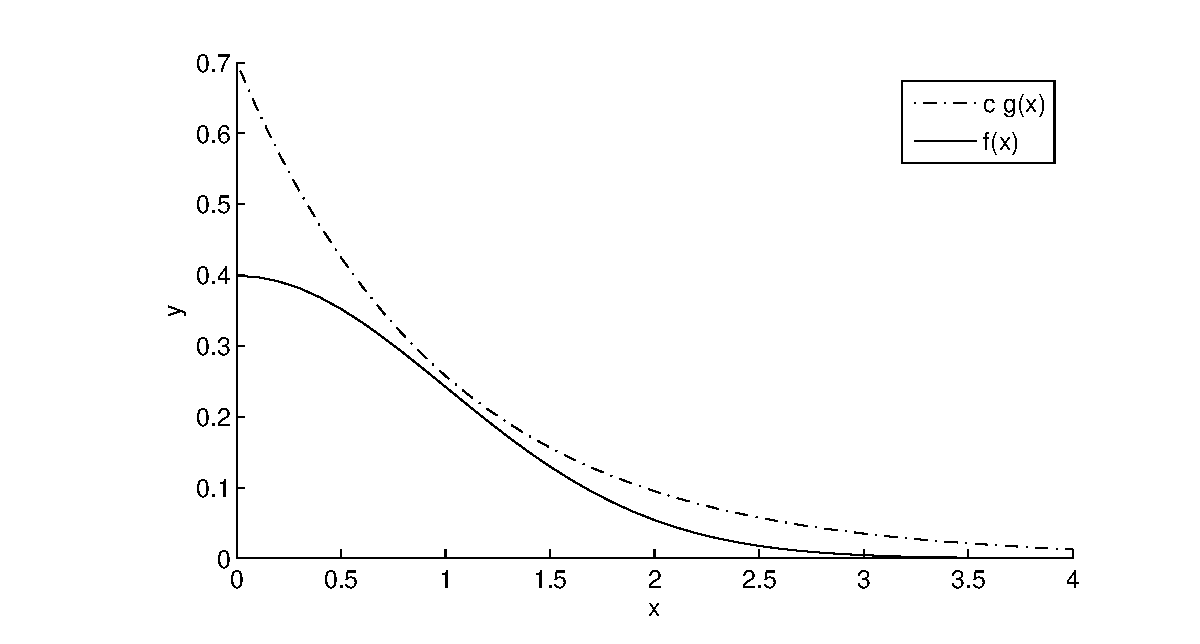
\includegraphics[width=1.0\textwidth]{figures/rejection_sampling.eps}
\caption[]{Rejection sampling of a half-normal distribution using an exponential distribution and a scaling constant $c = 0.7$.}
\label{app:fig:rejection_sampling}
\end{figure*}

Figure \ref{app:fig:rejection_sampling} shows  this for sampling from a half-normal distribution $f(x) = \sqrt{\frac{2}{\pi}} \exp(-\frac{x^2}{2}),~ x \geq 0$ using and exponential utility distribution $g(x) = \exp(-x), ~x \geq 0$ and a constant $c = 0.7$.

On average, rejection sampling takes $c$ iterations to accept a sample. This means that the smaller $c$ is, the more efficient rejection sampling is\,\citep{Knuth1997b}.

Rejection sampling is used to sample from a Poisson and Gamma distribution.

% VIVA Q: $f$ might not be known explicitly

\section*{Poisson distributed random numbers}
% references: Atkinson1979, Ahrens + Dieter1974, Ahrens + Dieter1982, Press2007, Knuth1997b
% Multiplication method: \cite[p.~137]{Knuth1997b}
% Poisson rejection method: \cite{Atkinson1979}

The Poisson random number generation is divided into three domains depending on $\lambda$. For small values, $\lambda < 30$, the multiplicative method as described for example by \citet{Knuth1997b} or \citet{Devroye1986} is used. The multiplicative method scales linearly with $\mu$ is thus only acceptable for small values of $\mu$. The generator exploits straightforward that the inter-arrival times are from the exponential distribution with mean $\lambda$\,\citep{Knuth1997b, Devroye1986}:\vspace{9mm}

{\setstretch{0.95}
\begin{lstlisting}[caption={Multiplicative method to sample from a Poisson distribution\,\citep{Devroye1986}.}, label=alg:poisson_multiply_method]
Let $x=0$, $sum = 0$;

while $sum  < \lambda$ do:
     sample $e$ from the exponential random number $E$;   
     $sum = sum + e$;
     $x = x + 1$;
end; 

return $x$;
\end{lstlisting}
}

If $30 < \lambda \leq100$ then rejection sampling is applied\,\citep{Atkinson1979}. The rejection method uses a linear approximation of $\mu^{-1}$. Due to the chosen constants, this approximation deteriorates if $\mu < 30$. Numerical studies conducted by \citet{Atkinson1979} indicate that the run-time of the rejection method is independent of $\mu$ and for values $\mu > 30$ it indicates the rejection method is faster than the multiplication method.

\subsubsection*{Stirling's approximation}
The rejection scheme proposed by \citet{Atkinson1979} requires the computation of $\ln(n!)$. Computing first the factorial and then the logarithm poses the problem that the factorial for even moderate values of $n$ is out of the range of 32-bit or 64-bit value stored in a computer. However, one can compute $\ln(n!)$ directly based on Stirling's approximation\,\cite{Knuth1997a}:

\begin{equation*}
n! \simeq \sqrt{2 \pi n} \; \left(\frac{n}{\mathrm e}\right)^{n},\qquad n\to\infty~.
\end{equation*}

Following \citet{Knuth1997a}, the Stirling sequence to compute $\ln (n!)$ can be written as:

\begin{equation*}
\ln(n!) = (n + \frac{1}{2}) \ln(n) - n + \sigma + \sum_{1 < k \leq m} \frac{B_k(-1)^k}{k (k - 1) n^{k - 1}} + O (\frac{1}{n^m})~,
\end{equation*}

where $B_k(n)=n^{k}-\sum_{m=0}^{k-1}\binom mk\frac{B_m(n)}{k-m+1}$ is the $k$-Bernoulli number, and $\sigma$ a canstant with $e^{\sigma} = \sqrt{2 \pi}$. This expression can be written as:

\begin{equation*}
\ln(n!) = n  \ln(n) + n + \frac{1}{2} \ln (2 \pi n) + \sum_{1 < k \leq m} \frac{B_k(-1)^k}{k (k - 1) n^{k - 1}} + O (\frac{1}{n^m})~.
\end{equation*}

Stirling's approximation is accurate for large $n$. This can be compensated for by pre-computing values for small $n$ and stringing them in a look-up table or binary search tree. This gives the opportunity to balance pre-computation and estimation of $\ln(n!)$.  Assuming a binary search tree of depth 5 storing $2^5 = 32$ pre-computed values, approximating $\ln(n!)$ by:

\begin{equation*}
\ln(n!) \approx n \ln(n) + \tfrac12\ln(2\pi n) - n + \frac1{12 n} ~,
\end{equation*}

gives an error smaller than $\frac1{360 \cdot 33^3} \approx 7.73^{-8}$ which is on the order of single precision floating point machine precision and thus sufficient for single precision computations. Using:

\begin{equation*}
\ln(n!) \approx n \ln(n) + \tfrac12\ln(2\pi n) - n + \frac1{12 n} - \frac1{360 n^3}~,
\end{equation*}

the error is smaller than $\frac{1}{1260 \cdot 33^5} \approx 2.02^{-11}$.

Another method to compute the $n!$ for large values of $n$ is to use the gamma function $\Gamma$ since $n! = \Gamma(n+1)$\,\citep{Bronstein1997}. Furthermore, many mathematical libraries including the CUDA mathematical libraries include functions to compute the logarithm of the gamma function $\ln(\Gamma(n))$. This function is called \textsf{lgamma}.

For large values of $\lambda > 100$ the Poisson distribution is approximated by a normal distribution. The approximation by the Central Limit Theorem (CLT) is $\Phi (\frac{k - \lambda}{\sqrt{\lambda}})$ where $\Phi(k)$ denotes the cumulative distribution function of the standard normal distribution. Often, the continuity correction $\Phi (\frac{k + \frac{1}{2}- \lambda}{\sqrt{\lambda}})$ is used\,\citep{Yates1934}. However, while reducing the absolute error \citet{Molenaar1970} points out that the relative error in the tails is increased.
%Two approximations of the Poisson distribution by a normal distribution not suffering from this are: (i) the Wilson-Hilferty approximation $\Phi(3 \sqrt{k + 1} - \frac{1}{3} (k + 1)^{-\frac{1}{2}} - 3 (\lambda \sqrt{k + 1})^{\frac{1}{3}})$ and, (ii) the \citet{Freeman1950}  approximation $\Phi(2 \sqrt{k + 0.75} - 2 \sqrt{\lambda})$\,\citep{Molenaar1970, Molenaar1973a}. This raises the question of how good this approximation is which is shown in Table \ref{app:table:approx_binomial_by_normal}. All three approximations achieve a maximum absolute error of less than $10^{-4}$. However, the Wilson-Hilferty and Freeman-Tukey approximations achieve a higher cumulated probability with less than $10\%$ relative error than the CLT approximation.

% \begin{table}
% \centering
% \footnotesize
% \begin{tabularx}{\textwidth}{ @{} K  K  c @{}}
%    \toprule
%    
%    {Approximation} & {max error}& {less than 10\% relative error}\\
%    \cmidrule(r){1-1}\cmidrule(lr){2-2}\cmidrule(l){3-3}
% 
%    CLT & $9.3881 \times 10^{-4}$ & 0.9807 \\
%    Wilson-Hilferty & $4.1025 \times 10^{-4}$ &  0.9993 \\
%    Freeman-Tukey & $4.5534 \times 10^{-4}$ & 0.9941 \\
% 
% \bottomrule
% \end{tabularx}
% \caption{Absolute and relative error when approximating the Poisson distribution with a normal distribution for $\lambda > 100$ using the approximation given by the Central Limit Theorem (CLT), the Wilson-Hilferty approximation, and the Freeman-Tukey approximation. For the relative error the cumulated probability with a relative error of less than 10 \% is given.}
% \label{app:table:approx_binomial_by_normal}
% \end{table}
% 
% \begin{figure*}
% \centering
% \includegraphics[width=1.0\textwidth]{appendix/pictures/poisson_normal_approx.eps}
% \caption[]{Approximation of the Poisson distribution with a normal distribution for $\lambda = 100$.}
% \label{app:fig:binomial_normal_approx}
% \end{figure*}   

\section*{Gamma distributed random numbers}
% References: Marsaglia2000, Ahrens + Dieter1974, Press2007, Knuth1997b

The Gamma distribution has a scale and shape parameter. For $a > 0$ the Gamma distribution is given by:

\begin{equation*}
F(x) = \frac{a}{\Gamma(a)} \int_{0}^{x} t^{a-1} e^{-t} dt, ~~~x \geq 0~.
\end{equation*}

The $\Gamma$ distribution has an infinite peak at $0$ for $a < 0$ and special care has to be taken. However, using a special case of Stuart's Theorem circumvents this problem and samples from $\Gamma_{a + 1}$are sufficient to generate $\gamma_a = \gamma_{a + 1} U^{\frac{1}{a}}$ where $U$ is a uniform distributed random variable on $(0, 1]$. For values of $a > 1$ the {\it RNOR} generator by \citet{Marsaglia2000} is implemented.
%
%Special cases: $a = 1$ exponentail distribution with mean $\lambda = 1$, $a = 0.5$ normal distribution $\frac{1}{2} \mathcal{N}(0,1)$
%
% for values $a > 1$
%
% working principals of the RNOR generator:
% requires fast uniform generator
% based on rejection method (need to add a paragraph about that)
% augmented by squeezes (need to add a paragraph about that)
%
This is based on the rejection method augmented by the squeeze method. The latter is a refinement of rejection sampling introduced by \citet{Marsaglia1977} to reduce the number of iterations until a sample is accepted. While the rejection function uses only one envelope above the distribution to be sampled, the squeeze method adds a second envelope below:

\begin{equation*}
h_1(x) \leq f(x) \leq h_2(x)~.
\end{equation*}

The generic rejection sampling algorithm with squeeze is given in Listing \ref{alg:rejectionsampling_squeeze}:\vspace{10mm}


{\setstretch{0.95}
\begin{lstlisting}[caption={Rejection-sampling with squeeze\,\citep{Devroye1980}.}, label=alg:rejectionsampling_squeeze]
Let $accept = 0$;

do {
    sample u from a uniform distribution;
    sample $x$ from the distribution with density $g$;
    
    $w = u \cdot c \cdot g(x)$;
    
    $accept = (w \leq h_1(x))$;
    if $\neg accept$ then:
        if $w \leq h_2(x)$ then:
            $accept = (x \leq f(x))$;
        end
    end;    
} while($\neg accept$);

return $x - 1$;
\end{lstlisting}
}

% Stuart's theorem:
Let $Z$ and $Y$ be independent random variables $\Gamma_{a}$ distributed and $\beta_{b, a - b}$ distributed, respectively. Then $Z(1 - Y)$
 is from the $\Gamma_{a - b }$ distribution. The distribution $\beta_{1, a}$ is linked to the uniform distribution $1 - Y^{\frac{1}{a}}$ is uniformly distributed. Furthermore, if $U$ is a uniform random number on $(0, 1]$, then $1 - U$ is also uniform on $(0,1]$. Let $b = 1$ and substitute $a$ with $a + 1$, then $Z U^{\frac{1}{a}}$ is also from the $\Gamma_{a}$ distribution\,\citep{Stuart1962, Devroye1986}.

\section*{Beta distributed random numbers}
The Beta distribution has two shape parameters $\alpha > 0$ and $\beta > 0$. The Beta distribution is given by:

\begin{equation}
F(x) = \frac{x^{\alpha - 1}(1-x)^{\beta-1}}{B_{\alpha, \beta}}~,
\end{equation}

where

\begin{equation}
B_{\alpha, \beta} = \int_{0}^{1} x^{\alpha-1} (1-x)^{\beta-1} dx = \frac{\Gamma(\alpha) \Gamma(\beta)}{\Gamma(\alpha + \beta)}~.
\end{equation}

Let $\Gamma_{\alpha, 1}$ and $\Gamma_{\beta, 1}$ be independent Gamma distributed random variables. Then the Beta distribution is linked to the gamma distribution such that $\frac{\Gamma_{\alpha,1}}{\Gamma_{\alpha, 1} + \Gamma_{\beta,1}}$ is from the Beta distribution $B_{\alpha, \beta}$ \cite{Devroye1986}.

So one may simply generate a beta random number from three Gamma distributed random numbers. However, to increase efficiency, Beta distributed random numbers are generated using the rejection sampling scheme by \citet{Cheng1978}.

%\bibliographystyle{IEEEtran}
\bibliographystyle{plainnat}
\bibliography{paper.bib}

\end{document}


